\documentclass[conference]{IEEEtran}
\IEEEoverridecommandlockouts
% The preceding line is only needed to identify funding in the first footnote. If that is unneeded, please comment it out.
\usepackage{cite}
\usepackage{amsmath,amssymb,amsfonts}
\usepackage{algorithmic}
\usepackage{graphicx}
\usepackage{textcomp}
\usepackage{changepage}
\usepackage{xcolor}
\def\BibTeX{{\rm B\kern-.05em{\sc i\kern-.025em b}\kern-.08em
    T\kern-.1667em\lower.7ex\hbox{E}\kern-.125emX}}
\begin{document}

\title{\emph \textbf Frequency of x in Sorted array using Divide and
conquer algorithm.\\

 
}

\author{\IEEEauthorblockN{Sarthak IIT2019114}
\IEEEauthorblockA{\textit{IV Semester} \\
\textit{B.Tech. in IT }\\
IIIT Allahabad\\
}
\and
\IEEEauthorblockN{Kaustubh Gangwar IIT2019115}
\IEEEauthorblockA{\textit{IV Semester} \\
\textit{B.Tech. in IT }\\
IIIT Allahabad\\}
\and
\IEEEauthorblockN{Harsh Singh IIT2019116}
\IEEEauthorblockA{\textit{IV Semester} \\
\textit{B.Tech. in IT }\\
IIIT Allahabad\\}


}

\maketitle
\textbf{\emph{Abstract - In this paper, we have devised an algorithm to Count number of occurrences (or frequency) of x in a given sorted array arr[] using divide and conquer algorithm.\\ \\
Keywords — binary search, frequency, divide, conquer}}\\






\section{Introduction}
Divide and Conquer is an algorithm design paradigm in which we recursively break down a problem into two or more sub-problems of the same or related type, until these subproblems become simple enough to be solved directly. \\ \\
The solutions to the sub-problems are then combined
to give a solution to the original problem.
The divide-and-conquer paradigm is often used to find an optimal solution of a problem in which we recursively simplify the problem by decreasing the constraints of a subproblem and selecting/ dis-selecting a given subproblem based on some conditions. \\ \\
Binary search is a search algorithm that finds the position of a target value within a sorted array. Binary search compares the target value to the middle element of the array. If they are not equal, the half in which the target cannot lie is eliminated and the search continues on the remaining half, again taking the middle element to compare to the target value, and repeating this until the target value is found. If the search ends with the remaining half being empty, the target is not in the array. \\ \\
In each step, the algorithm compares the input element x with the value of the middle element in array. If the values match, return the index of the middle. Otherwise, if x is less than the middle element, then the algorithm recurs for left side of the middle element, else recurs for the right side of the middle element. Since the given array is sorted, we came up with the idea of using binary search.\\


\section{Algorithm}

\subsection{Algorithm Description}

Since the array is sorted, all occurrences of x will be adjacent. So, run a linear scan to find all instances of x to the left of the found index, and its right. The worst-case time complexity of this solution remains O(n) . The worst case happens when all the array elements are the same as the given number.\\ \\
We can easily solve this problem in O(log(n)) time by modifying the binary search algorithm . The idea is to find the index of the first and last occurrence of the given number and return one more than the difference between two indices because the array is sorted and all the x’s are between these two indices only. \\ \\

So, the steps used in this algorithm are : \\ \\
1) Use Binary search to get index of the first occurrence of x in arr[]. Let the index of the first occurrence be i. \\ \\ 
2) Use Binary search to get index of the last occurrence of x in arr[]. Let the index of the last occurrence be j.\\ \\
3) Return (j – i + 1); //And This will be the frequency of x.

\subsection{Algorithm Analysis}

As the given array is already sorted so we will find the first occurrence of x in arr[] using the function search() by passing the array arr[] , n i.e. size of array , x and 1. \\  If the returned value is -1 that means the element is not present in array and we will stop our algorithm here and if it is not -1 then we will find the last occurrence of x in array arr[] by using search() function again but this time we will pass 0 instead of 1 in flg value to get the last occurrence of x. \\  So, after getting the first and last occurrence of x in arr[] , the number of occurrence of x will be last - first + 1.

\subsection{PSEUDO CODE}\label{AA}
Pseudo Code for function search(int arr[],int N,int x,int flg)
We will pass array arr[], its size N, value of x, and flg value as 1 if we want to find first occurrence of x else 0 if we want to find last occurrence of x. \\
We will initialize the result by -1 and while loop till the search space is exhausted find the mid-value in the search space and compares it with the target if the target is found, update the result if flg is 1 go on searching towards the left (lower indices) else go on searching towards the right (higher indices) if the target is less than the middle element, discard the right half if the target is more than the middle element, discard the left half. In the end return the result.

int low = 0; \\
int high = N - 1; \\
int result = -1;\\
while ($low <= high$)\\
{\\
int mid = (low + high)/2;\\
if (x == arr[mid])\\
result = mid;\\
if (flg)\\
high = mid - 1;\\
else\\
low = mid + 1;\\
else if ($x < arr[mid]$)\\
high = mid - 1;\\
else\\
low = mid + 1;\\
}\\
return result;\\ \\
PSEUDO CODE for main() : \\ \\
int first = search(arr, n, x, 1);\\
if (first != -1){\\
int last = search(arr, n, x, 0);\\
int count = last - first + 1;\\
print(count) \\
}\\
else\\
print("Element not found in the array.");\\

\subsection{Time Complexity}

While Finding the First and Last Occurrence of x if the complexity of the entire Algorithm is T(n) where n signifies number of elements, we are actually reducing the list to half i.e T(n/2) in every step of the loop along with some constant time (O(1) for reference) needed to find middle index and do comparisons.
Hence Time Complexity of Binary
Search = $T(n) = T(n/2) + O(1)$
Let the iteration in Binary Search terminates
after k iterations.
At each iteration, the array is divided by
half.

So let’s say the size of search space at any
iteration is n\\
\textbf{At Iteration 1,}\\
size of search space = n\\
\textbf{At Iteration 2,}\\
size of search space = n/2\\
\textbf{At Iteration 3,}\\
size of search space = (n/2)/2 = n/4\\
\textbf{At Iteration 4,}
size of search space = (n/2 )/2=n/8 \\

Therefore, after Iteration 4 \\
size of search space = n/16 \\ \\ 
Hence size of search space after k iteration
is = $n/(2^k)$ \\
Also, we know that after k divisions, the size of search space becomes 1. \\ \\
Therefore size of search space = $n/2^k$ = 1 \\
$ n = 2^k $ \\ 
Applying log function on both sides: \\ 
$ log(n) = log(2^k)$ \\ 
$ log(n) = k log(2)$ \\
$ log(n) = k$ \\

Therefore,
$k = log(n)$ \\ \\ 
Hence, the time complexity of first index
search is $log(n)$. \\ 
Similarly time complexity of Rightmost
search is $log(n)$. \\ 

\begin{figure}[h!]
\centerline{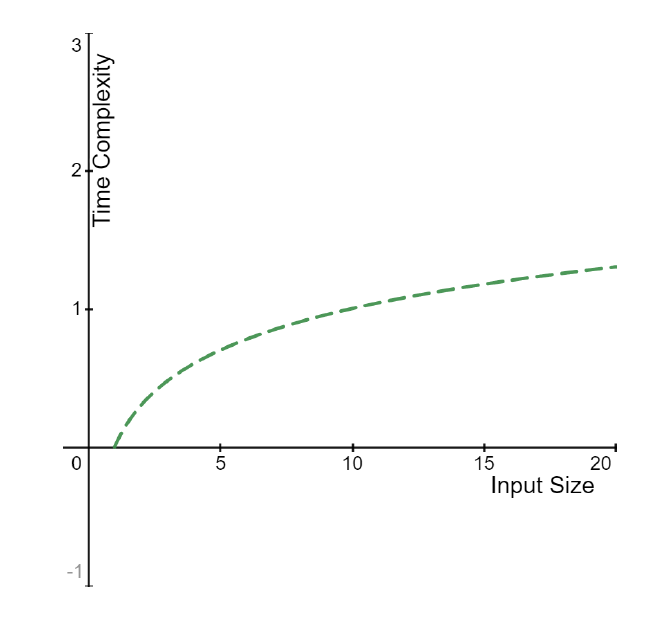
\includegraphics[width=85mm,height=80mm ]{TC.png}}
\caption{Input Size vs Time complexity.}
\label{fig2}
\end{figure} \\
\textbf{
Hence the complexity of finding freq of x is $log(n)$.} \\ \\

\subsection{SPACE COMPLEXITY} \\
\textbf{Space required for searching is O(1)} because we just use some variables which come under O(1) or constant space
complexity. \\ 
Only Space required is for storing the array arr[] of size n which will be O(n).

\section{CONCLUSION}
In this program we learn how binary search can be used in various aspects of problem solving for lesser running time and lesser memory. We also learn about how binary search works on the phenomenon of divide and conquer algorithm.
We analyze that binary search algorithm works on the idea of neglecting half of the list on every iteration. It keeps on splitting the list until it finds the value it is looking
for in a given list. \\ \\
A binary search algorithm is a quick upgrade to a simple linear search algorithm.\\
Thus in aspect of time and space complexity Binary search Algorithm is better than linear Search algorithm. \\
We have also shown above how worst case time complexity of binary search is logarithmic by taking one simple
illustration.




\begin{thebibliography}{00}

\bibitem{b1} Introduction to Algorithms by Cormen,Charles,Rivest and Stein.https://web.ist.utl.pt/ fabio.ferreira/material/asa

\bibitem{b2} Introduction to divide and conquer technique: https://www.geeksforgeeks.org/divide-and-conquer-algorithm-introduction
\bibitem{b3} Binary Search Algorithm :    https://en.wikipedia.org/wiki/Binary_search_algorithm
\end{thebibliography}
\vspace{12pt}


\end{document}
